% Name: Complex plane
% Description: A complex number z = a + bi as a point and an arrow, with its modulus, its argument, and its conjugate reflected below the real axis.
% Tags: complex numbers, Argand diagram, modulus, argument

\usetikzlibrary{arrows.meta, angles, quotes}

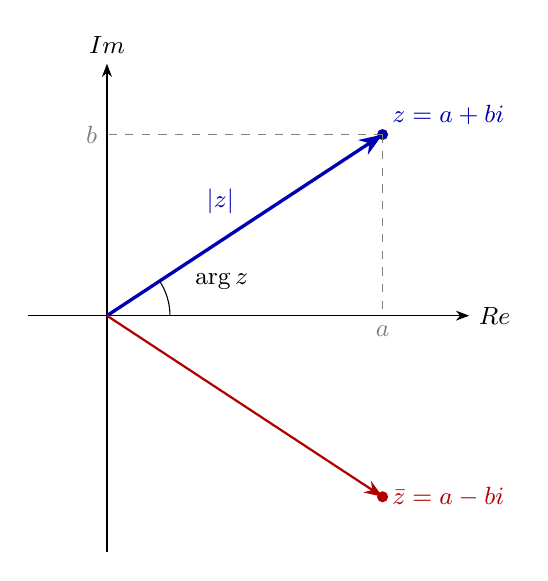
\begin{tikzpicture}[>={Stealth}, every node/.style={font=\small}]
  \draw[->] (-1,0) -- (4.6,0) node[right] {$\operatorname{Re}$};
  \draw[->] (0,-3) -- (0,3.2) node[above] {$\operatorname{Im}$};
  \coordinate (O) at (0,0);
  \coordinate (X) at (1,0);
  \coordinate (Z) at (3.5,2.3);
  \draw[->, very thick, blue!70!black] (O) -- node[above left] {$|z|$} (Z);
  \fill[blue!70!black] (Z) circle (2pt) node[above right] {$z = a + bi$};
  \draw[dashed, gray] (Z) -- (3.5,0) node[below] {$a$};
  \draw[dashed, gray] (Z) -- (0,2.3) node[left] {$b$};
  \pic[draw, "$\arg z$", angle eccentricity=1.9, angle radius=8mm] {angle = X--O--Z};
  \draw[->, thick, red!70!black] (O) -- (3.5,-2.3);
  \fill[red!70!black] (3.5,-2.3) circle (2pt) node[right] {$\bar{z} = a - bi$};
\end{tikzpicture}
